\documentclass[12pt]{article}
\usepackage[utf8]{inputenc}
\usepackage{geometry}
\geometry{
 a4paper,
 total={170mm,257mm},
 left=20mm,
 top=25mm,
 }
\usepackage{layout}
\usepackage{amsmath, amssymb}
\usepackage{graphicx}
\usepackage{cleveref}
\usepackage{float}
\usepackage{pdfpages}
\usepackage[framed, numbered]{matlab-prettifier}
\usepackage{romanbar}

\setlength{\parskip}{1em}

\title{Checkpoint 3\\Telescopic Radio Antenna Design\\Design For Vibration\\Group 3}
\author{Tate Halsey\\Serop Kelkelian\\Dominic Watson}
\date{\today}

\begin{document}
\pagenumbering{gobble}%
\maketitle
\newpage

\tableofcontents
\newpage

\section{Abstract}
\pagenumbering{arabic}
Our team has been tasked with designing a telescopic radio antenna to pick up (FM) signals for a portable radio. The goal of this report is to ensure that the material and geometry of the antenna is functional without fail, whilst satisfying the manufacturer’s design requirements. Approaching this specification with no restriction, the antenna is broken up into 6 segments. Upon full extension, the length of the antenna is 69.5 centimeters; fully retracted length measures out to approximately 11.5834 centimeters. Calculated tube wall thickness of the antenna is 0.04167 centimeters, while the maximum diameter is 0.5 centimeters. In order to satisfy design requirements and functionality, the material chosen for this antenna was stainless steel 304. The density of the antenna comes out to 8000 kg/m$^3$ [2]. Calculating change in stress over change in strain, the elastic modulus of the antenna is 200 GPa [2]. The yield strength is 207 MPa [3]. Maximum normal stress for the antenna under a given loading is 167.815 MPa. The margin of security, or safety factor, for the antenna is 1.2335 (dimension-less). Maximum deflection was 0.067103 meters which occurred at the end of the antenna, at a length of 0.0695 meters. The fundamental frequency of vibration is 235.69 Hz. Total mass of the antenna comes out to 0.0182 kg. Total cost of raw materials needed to assemble the antenna was \$0.0042 USD.
\newpage

\section{Introduction}
We have been tasked to design a telescopic antenna that would serve as an (FM) signal receiver for portable radios. This task requires a specific design geometry which includes: number of sections, length, and thickness. All of which must meet the given design requirements as well as successfully pick up FM radio signals. In [1], the frequency for (FM) radio signals ranges from 87 to 108 (MHz). To find the related wavelength, $v=\lambda f$, the frequency range was divided by the speed of light in a vacuum. The calculated wavelength for an (FM) radio signal ranges from 2.78 to 3.45 meters. Understanding that the design is a quarter-wave antenna and can only pick up one-quarter of the wavelength of the intended (FM) radio signal, the admissible length ($L$) for the antenna ranges from 0.695 to 0.8625 meters.
\newpage

\section{Design}

\begin{figure}[H]
\centering
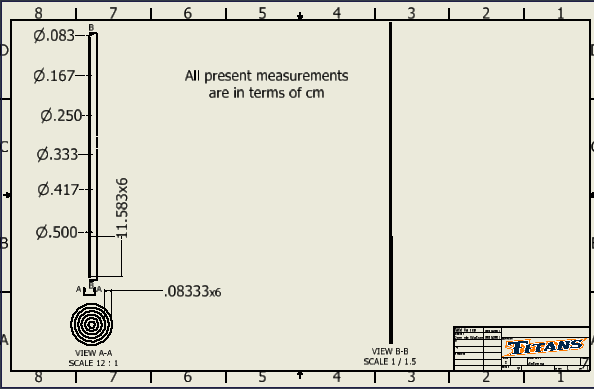
\includegraphics[height= 11cm, width= 15cm]{Antenna.png}
\caption{CAD Drawing of Antenna}
\label{CadDrawingAntenna}
\end{figure}

The material chosen for this design is stainless steel 304. This material has a density of 8000 kg/m$^3$ [2], an elastic modulus of 200 GPa [2], and a yield strength of 207 MPa [3]. The antenna design has 6 segments that are all 11.583 centimeters in length, for a total length of 69.5 centimeters. The segments decrease in radius moving inwards by 0.08333 m. The diameter of the largest segment is $0.5$ centimeter.
\newpage

\section{Static Stress Analysis}
In the process of deriving our static stress analysis, there were a plethora of problems to be solved leading to our result. The given free-body diagram, Figure \ref{FreeBodyDiagram} helped create a shear-force and bending-moment diagram, Figures \ref{ShearForceDiagram} and \ref{BendingMomentDiagram}, respectively.

\begin{figure}[H]
\centering
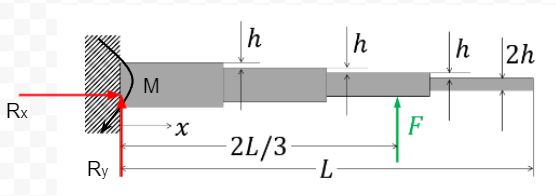
\includegraphics[height= 4cm, width= 10.5cm]{freebody.png}
\caption{Free Body Diagram}
\label{FreeBodyDiagram}
\end{figure}

\begin{figure}[H]
\centering
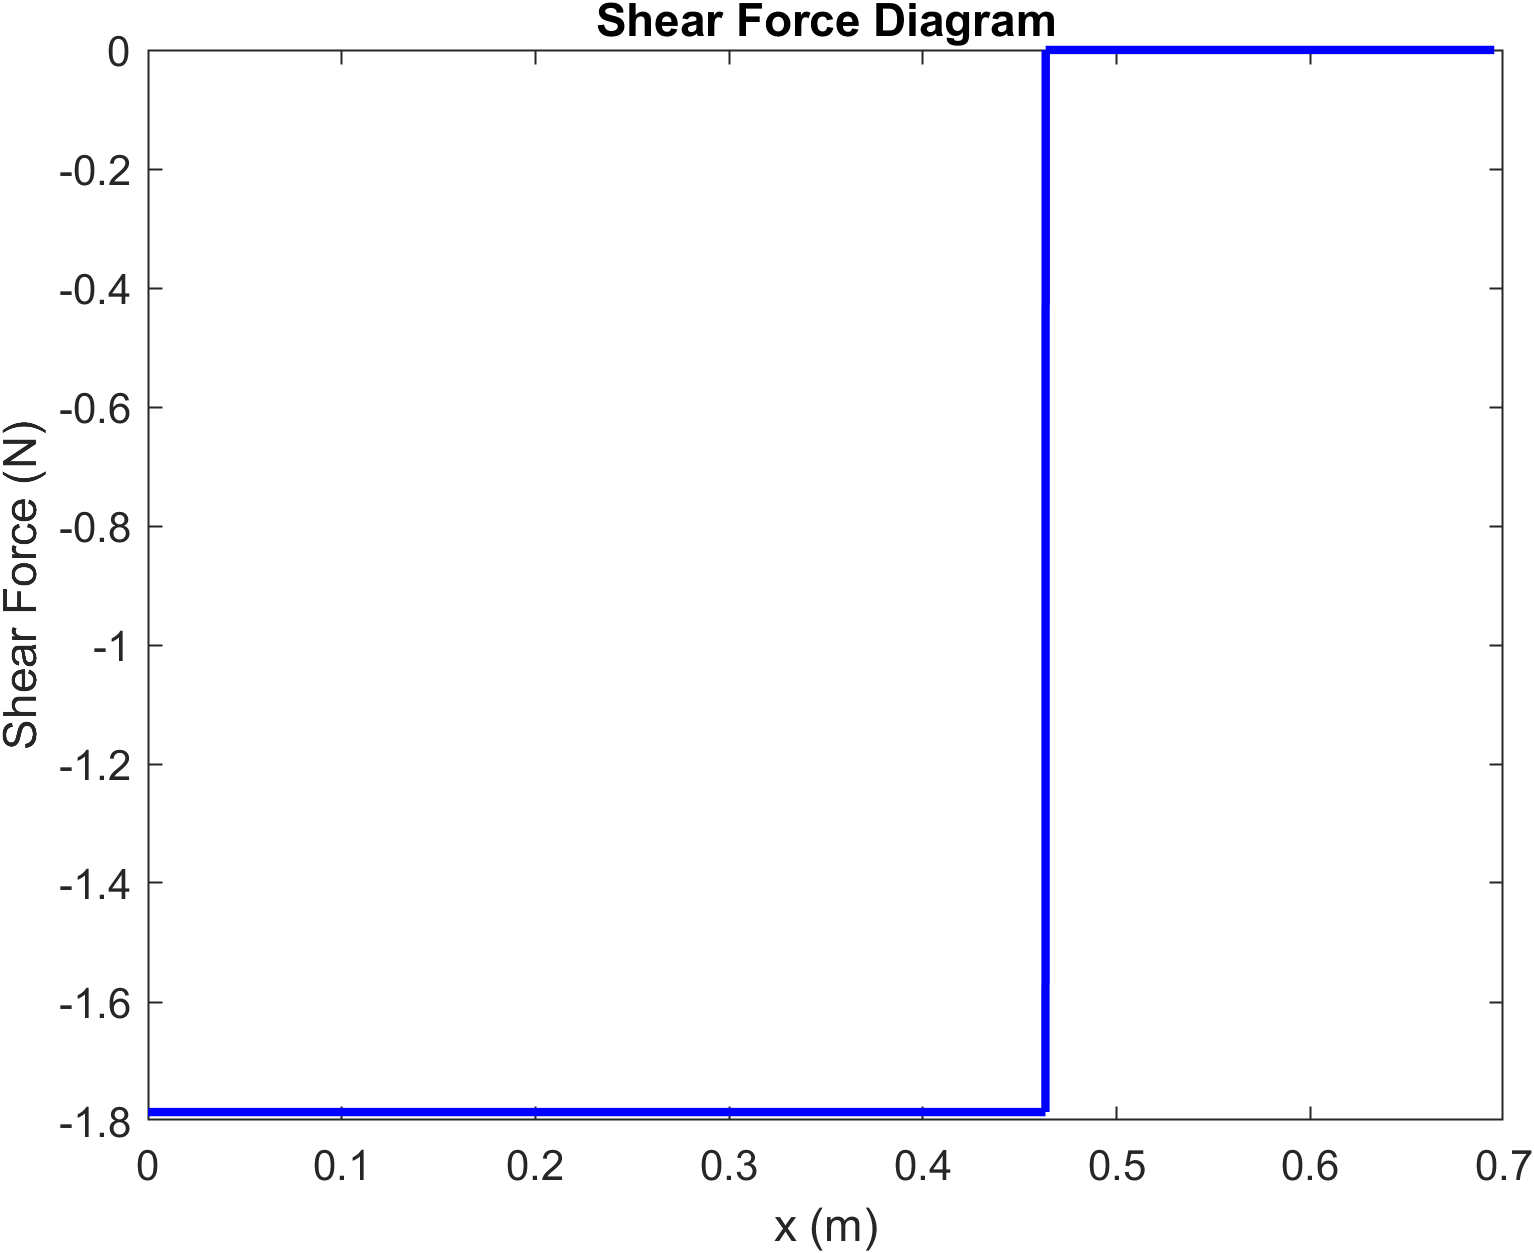
\includegraphics[height= 9.5cm, width= 12.5cm]{curve_Shear_Force.png}
\caption{Shear Force Diagram}
\label{ShearForceDiagram}
\end{figure}

\begin{figure}[H]
\centering
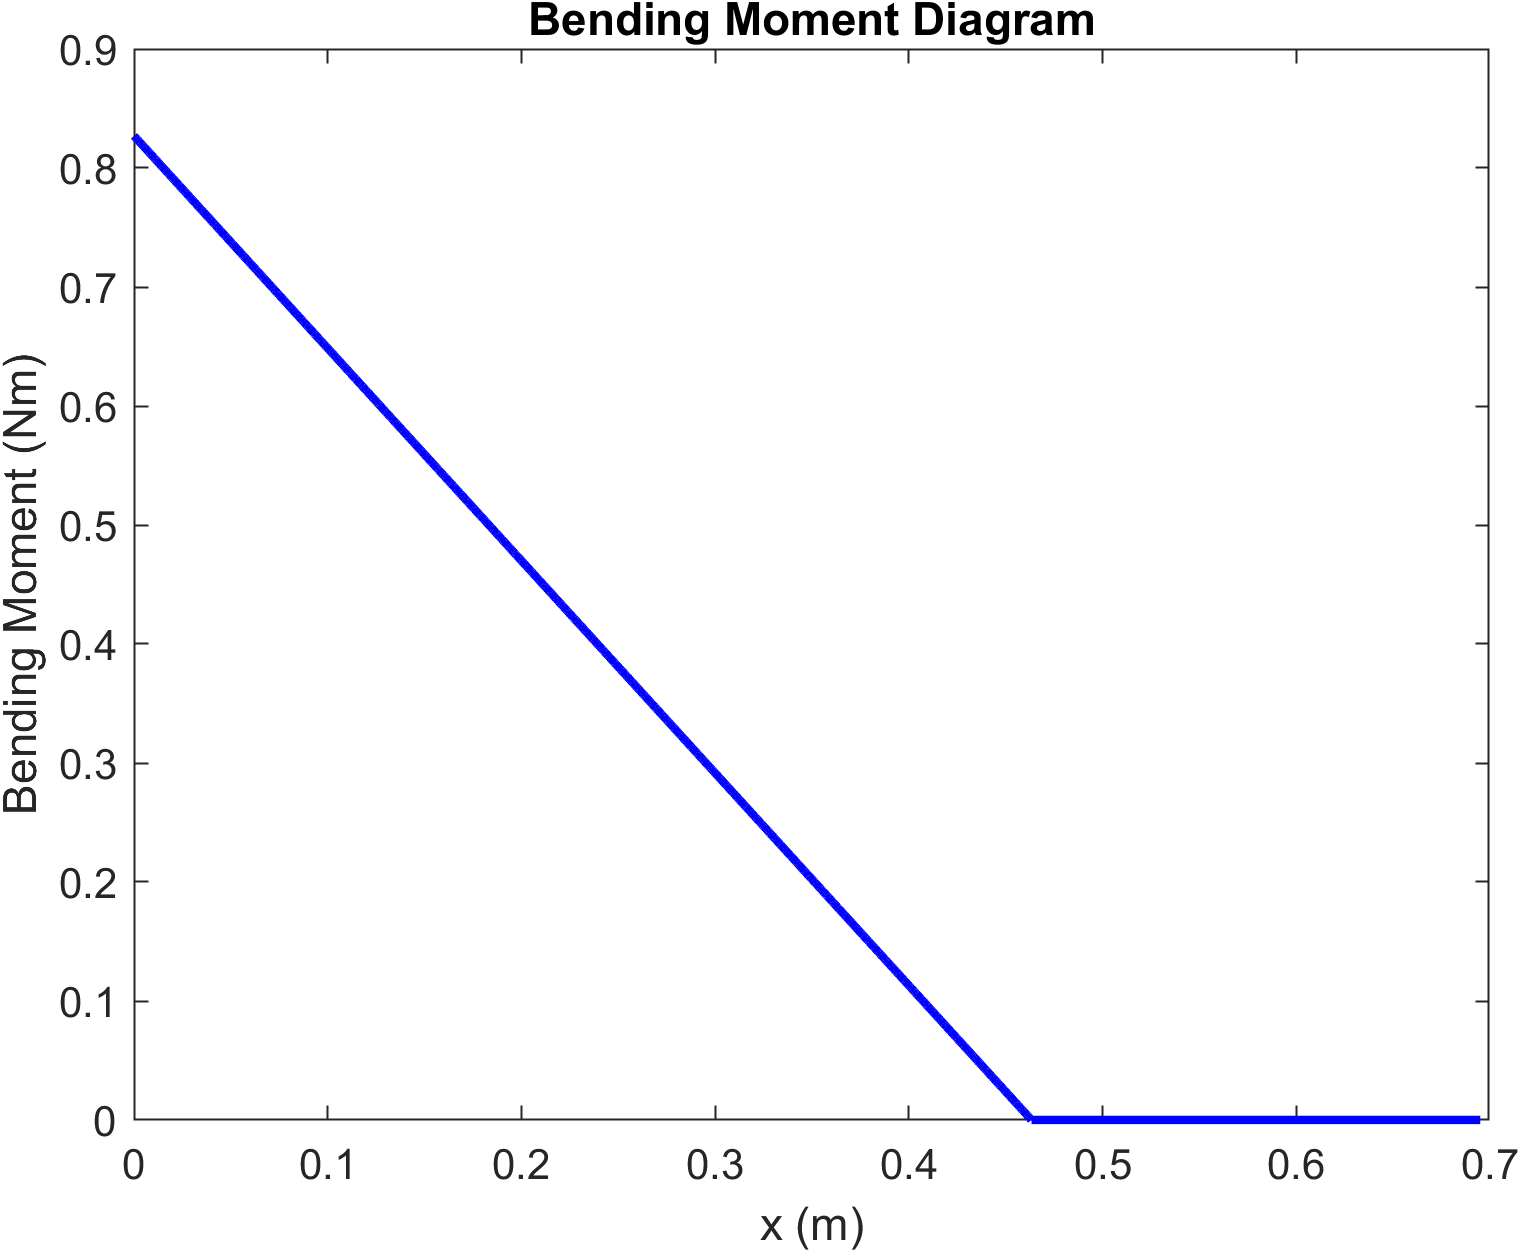
\includegraphics[height= 9.5cm, width= 12.5cm]{curve_Bending_Moment.png}
\caption{Bending Moment Diagram}
\label{BendingMomentDiagram}
\end{figure}

\setlength{\parindent}{0cm}
This stage was simply recognizing that the arbitrary concentrated force $F$ was the single external force acting on the beam, so the only internal reaction force $R_y$ must be equal in magnitude but opposite in direction as to maintain static equilibrium. This concept stayed relevant in the bending moment diagram as well for the only moment was caused by the single concentrated force $F$ at a distance $2L/3$, where $L$ is the full length of the antenna and is equal to 0.695 meters, therefore there must be a moment at the support equal in magnitude but opposite in direction to maintain static equilibrium. Now with this first step out of the way, the next step was to derive a symbolic equation for $M(x)$ using the Laplace transform technique. 

Originally, we were given the equation
\begin{equation}
    \centering
    M''(x) = w(x),
\end{equation}
where $M''(x)$ is the second derivative of the bending moment with respect to x and $w(x)$ is the transverse force per unit length applied to the antenna as a function of $x$.

After deciding on a form for $w(x)$  to take, our work arrived us to
\begin{equation}\label{eq:TransverseForce}
    \centering
    w(x) = F\delta(x - \frac{2L}{3}).
\end{equation}
We then took the Laplace transform of both sides of Equation~\eqref{eq:TransverseForce}, resulting in
\begin{equation}
    \centering
    s^2 \mathcal{L}[M(x)] - sM(0) - M'(0) = \mathcal{L}[w(x)].
\end{equation}
After inputting values gained from the bending moment graph, move appropriate values to the right side of the equation and arrive at the equation
\begin{equation}
    \centering
    s^2 \mathcal{L}[M(x)] = F\mathcal{L}[\delta(x - \frac{2L}{3})] + \frac{2FL}{3}{s} - F.
\end{equation}
At this point we are left with solving for the Laplace transform of the $w(x)$  function
\begin{equation}
    \centering
    s^2 \mathcal{L}[M(x)]=Fe^{-\frac{2L}{3}} + \frac{2FL}{3}{s} - F.
\end{equation}
Then divide both sides by $s^2$,
\begin{equation}
  \centering
  \mathcal{L}[M(x)] = \frac{Fe^{-2L/3 \cdot{s}}}{s^2} + \frac{2FL}{3} \cdot \frac{1}{s} - F \cdot \frac{1}{s^2}
  \end{equation}
 and take the inverse Laplace transform of both sides,
 \begin{equation}
  \centering
   M(x) = {F\mathcal{L}}^{-1}(\frac{e^{-2L/3 \cdot{S}}}{s^2}) + \frac{2FL}{3} \cdot \mathcal{L}^{-1}(\frac{1}{s})- F\mathcal{L}^{-1} (\frac{1}{s^2}).
  \end{equation}
 Finally, solve for the bending moment equation $M(x)$,
  \begin{equation}
  \centering
   M(x) = -Fx + \frac{2FL}{3} + F(x - \frac{2L}{3}) \cdot H(x - \frac{2L}{3}),
  \end{equation}
  where $F$ is the concentrated force, $L$ is the length of the antenna, and $H(\;)$ is the Heaviside function.
  
Once the derivation was complete, it was onto plotting the relevant equations for the maximum normal stress. The maximum vertical distance from the neutral surface within the cross-section, $C(x)$ is found in Figure \ref{MaximumVerticalDistance} and given by the equation,
\begin{equation}
  \centering
   C(x) = Nh-\sum_{n=1}^{N-1}h \cdot{H(x - \frac{n \cdot{L}}{N}}),
  \end{equation}
where $N$ is the number of segments present on the antenna, $h$ is the thickness of each antenna piece, and $n$ is the summation index.

Next is $I(x)$, seen in Figure \ref{SecondMomentArea}, which is the second moment of area of the cross-section and given by the equation:
\begin{equation}
  \centering
   I(x) = I - \sum_{n=1}^{N-1}\frac{\pi}{4}h^4((N - n + 1)^4 - 2(N - n)^4 +(N - n - 1)^4)H(x - \frac{n\cdot{L}}{N}).
  \end{equation}
 Finally, the normal stress $\sigma(x)$ shown in Figure \ref{MaximumNormalStress}, is given by the equation,
 \begin{equation}
  \centering
   \sigma(x) =  \frac{|M(x)|C(x)}{I(x)}.
  \end{equation}
  With both these graphs available for inspection and their necessary code refined, important pieces of data can be found. One of interests is the location of the maximum normal stress, which occurred at the length 0.3475 meters, therefore the exact numerical value for normal stress is given by the equation,
  \begin{equation}
  \centering
   \sigma(x) = \frac{|-Fx + \frac{2FL}{3} + F(x - \frac{2L}{3})H(x - \frac{2L}{3})|Nh - \sum_{n=1}^{N-1}h \cdot H(x -\frac{n \cdot{L}}{N})}{I - \sum_{n=1}^{N-1}\frac{\pi}{4}h^4((N - n + 1)^4 - 2(N - n)^4 +(N - n - 1)^4)H(x - \frac{n\cdot{L}}{N})},
  \end{equation}
  when $x$ is equal to 0.3475 meters. Then once inputted with appropriate constants, it resolves into approximately 167.8 MPa. With this approximate value our safety factor is found to be 1.2335 (dimension-less).

\begin{figure}[H]
\centering
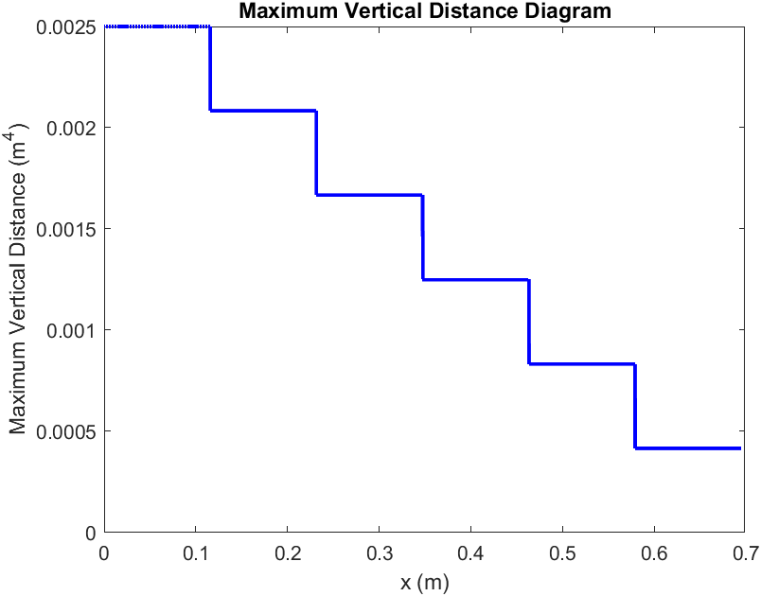
\includegraphics[height= 9.5cm, width= 12.5cm]{Max_Vertical_Distance.png}
\caption{Maximum Vertical Distance}
\label{MaximumVerticalDistance}
\end{figure}

\begin{figure}[H]
\centering
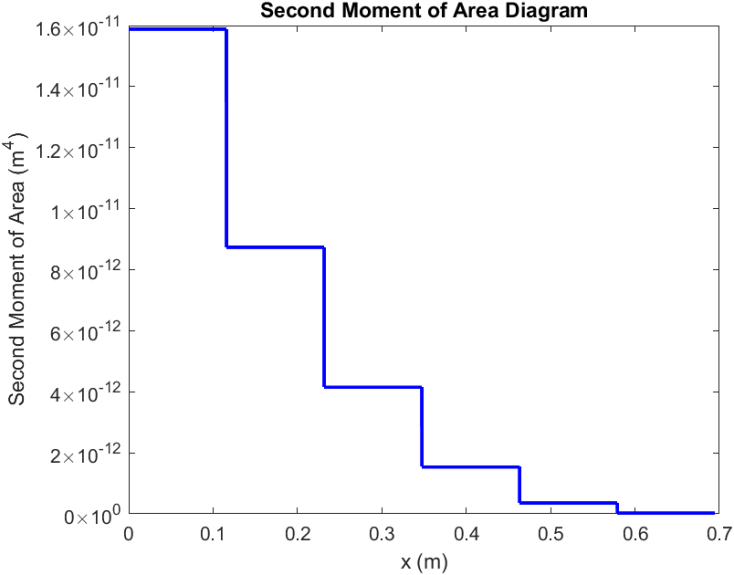
\includegraphics[height= 9.5cm, width= 12.5cm]{Second_Moment_of_Area.png}
\caption{Second Moment Area}
\label{SecondMomentArea}
\end{figure}

\begin{figure}[H]
\centering
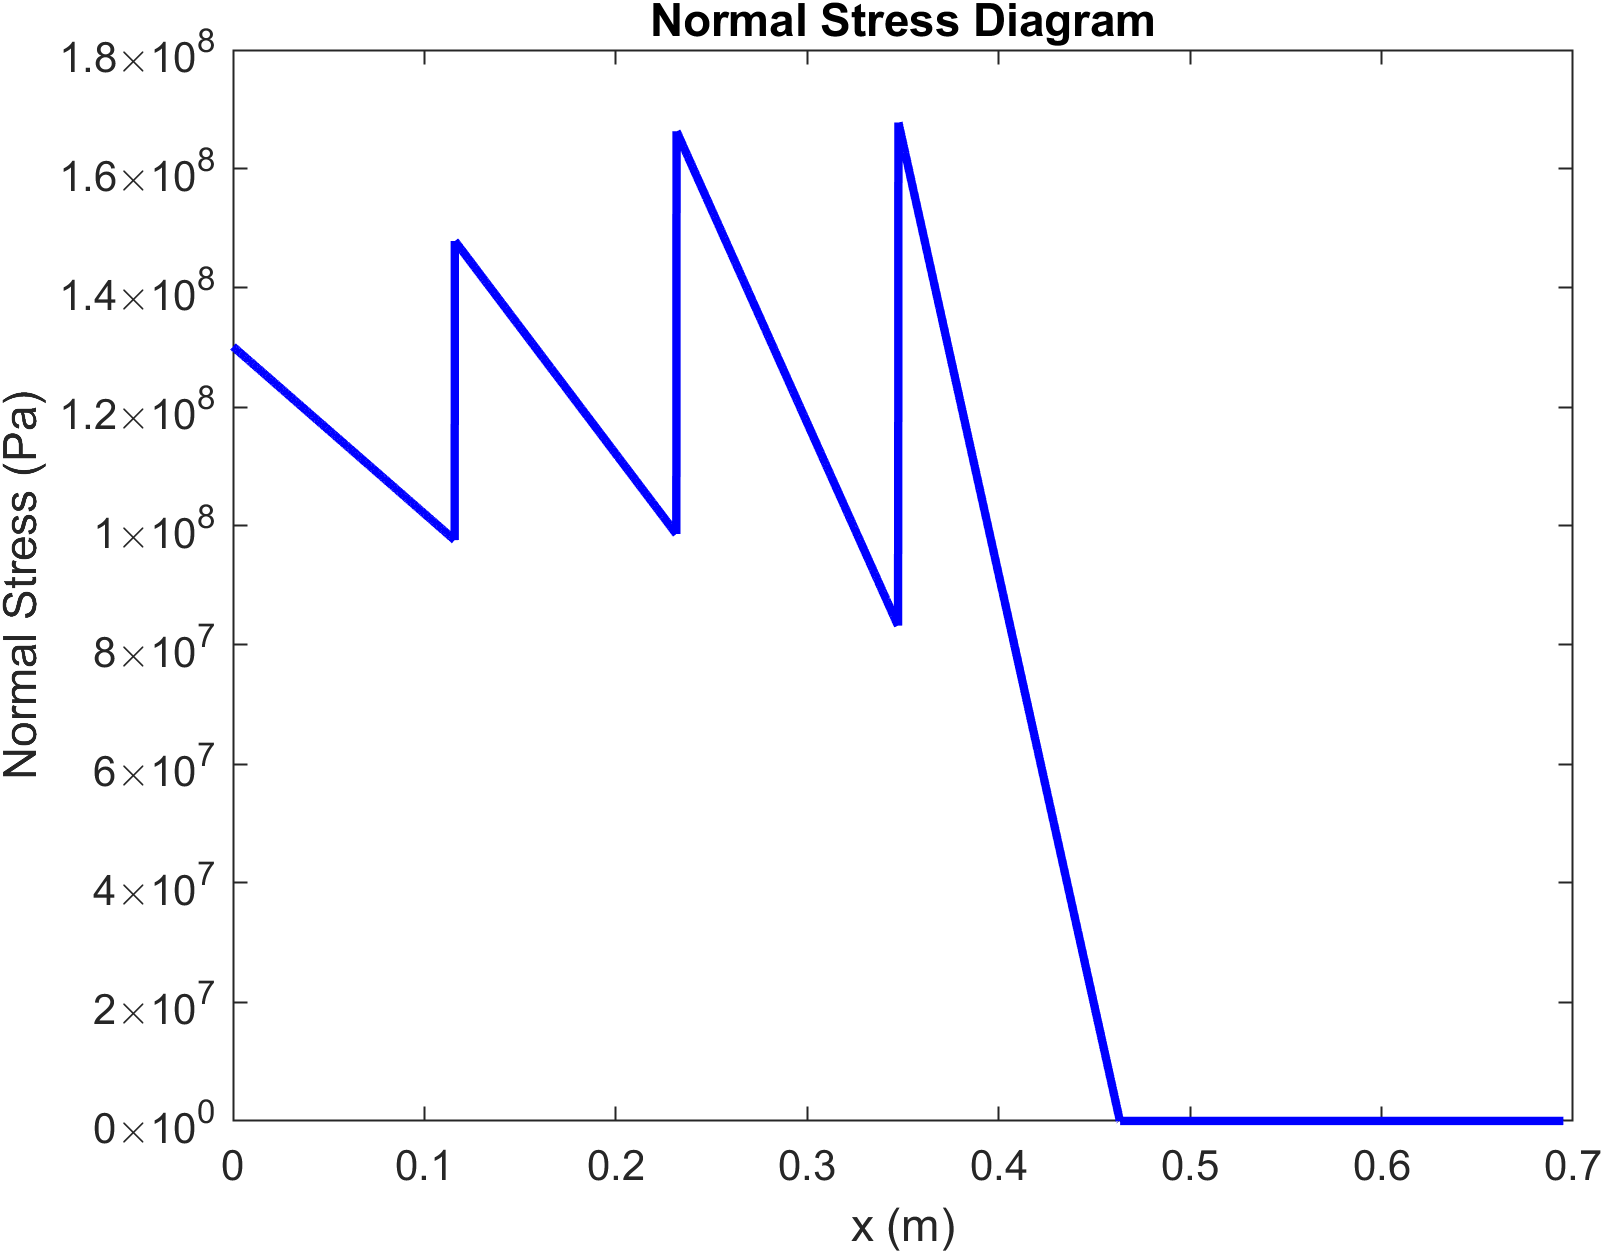
\includegraphics[height= 9.5cm, width= 12.5cm]{curve_Normal_Stress.png}
\caption{Maximum Normal Stress}
\label{MaximumNormalStress}
\end{figure}
\newpage

\section{Static Deflection Analysis}
While analyzing deflection under static conditions, we solved for the deflection curve using the Euler-Bernoulli beam equation. In order for the deflection curve to be the solution to the Euler-Bernoulli beam equation, the assumptions of Euler-Bernoulli beam theory must be met. First, the cross-sections must remain planar and normal to the longitudinal axis before and after deformation. Because it does not deform permanently, the cross-section is considered a rigid surface which means it can only rotate. The second assumption is that the beam is homogeneous and has a longitudinal plane of symmetry. Lastly, even though the beam has a slight curve after deformation, deflections are considered to be small and shear deformations are to be neglected.
\setlength{\parindent}{0cm}

Because these assumptions are met, we could use
\begin{equation}
    \centering
    \ EI(x)u''(x) = M(x),
\end{equation}
the Euler-Bernoulli beam equation to solve for the deflection curve. Here $E$ is the modulus of elasticity, $I(x)$ is the second moment of area, and $M(x)$ is the bending moment.

Isolating $u’’(x)$, we obtain 
\begin{equation}\label{eq:Deflection}
    \centering
    \ u''(x) = \frac{M(x)}{EI(x)}.
\end{equation}
The antenna is being modeled as a cantilever beam as the antenna is fixed on the supported end. The boundary conditions at $x = 0$ are given below:
\begin{equation}
    \centering
    u(0) = 0,\; \;u'(0) = 0.
\end{equation}
Solving for this problem analytically is much more difficult than solving for it numerically because $I(x)$ and $M(x)$ are both piecewise functions. As $N$, the number of segments increases, it becomes increasingly difficult to solve for this problem analytically.

The procedure for Euler’s method goes as follows. First, one must identify the dependent and independent variables. We are using Euler’s method to solve for the vertical deflection as a function of $x$, distance along the length of the beam. Thus, the independent variable is $x$ and the dependent variable is the vertical deflection. Next, we must discretize the independent variable. In this case, we will discretize $x$ into constant increments of $x$. After discretizing the independent variable, approximate all derivatives with finite difference quotients. We are solving for vertical deflection with respect to $x$. As the constant increments of $x$ get smaller, the approximation becomes more accurate because the numerical solution will get closer and closer to the analytical solution. Using a sufficiently small increment $\Delta{x}$, we could successfully model the behaviour of $u(x)$ everywhere. After modeling the behaviour of $u(x)$, use this equation 
\begin{equation}\label{eq:Eulersmethodu}
    \centering
    u_{n+1} = {u_n}\;+u_n'\; \Delta{x}
\end{equation}
to solve for quantities at $(n+1)^{th}$ point along the beam in terms of quantities at the $n^{th}$ point. In Equation~\eqref{eq:Eulersmethodu}, $u_{n+1}$ is the quantity at the subsequent point, $u_n$ is the quantity at the previous point, $u_n'$ is the derivative of the quantity at the previous point and $\Delta{x}$ is the length increment. Taking the finite difference quotient of $u'$ gives us
\begin{equation}
    \centering
    u_{n+1}' = u_n'\;+u_n''\; \Delta{x}
\end{equation}
which we used to calculate the deflection. The deflection was calculated over a set of $x$ values from 0 to the length of the antenna that increment by $\Delta{x}$. This makes it very time-efficient to solve this problem numerically using MATLAB. After constructing a numerical solution, we will run a convergence study to ensure that our numerical solution converges to the analytical solution. We will decrease $\Delta{x}$ by orders of magnitude until the numerical solution stops changing to the desired accuracy.

Once the derivation was complete, we modified the MATLAB script to include the deflection curve. The deflection curve was created to identify the single greatest deflection $|u|_{max}$ along the entire length of the antenna, and the point at which that deflection occurs. 

We wanted an answer within 0.0000001 meters of the exact answer. After running a convergence study we found the exact increment, \\

\centerline{$\Delta{x} = 0.000001$ m;}

we obtained a deflection curve shown in Figure \ref{DeflectionCurve}. According to Figure \ref{DeflectionCurve}, the greatest deflection was 0.067103 meters which occurred at a length of 0.695 meters. This is equal to the maximum value specified for the length of the antenna in the design requirements.

\begin{figure}[H]
\centering
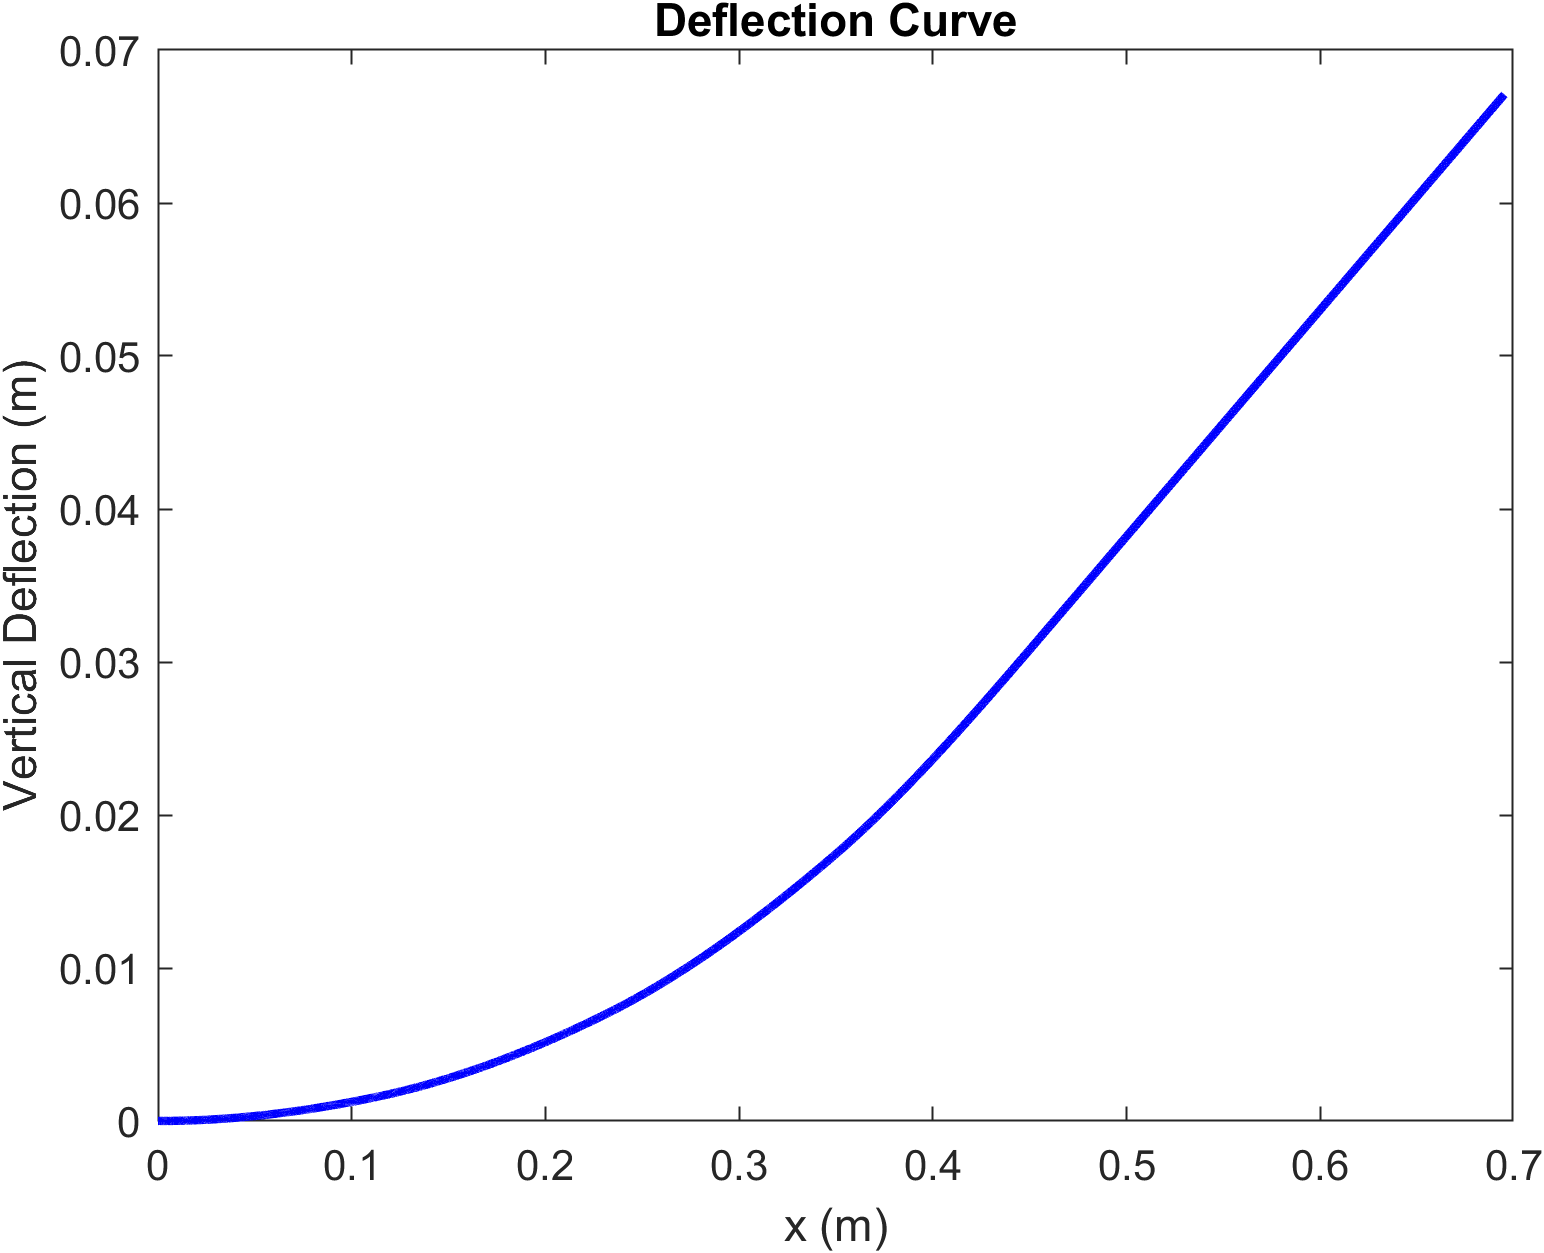
\includegraphics[height= 9.5cm, width= 12.5cm]{curve_Deflection_Curve.png}
\caption{Deflection Curve}
\label{DeflectionCurve}
\end{figure}
\newpage

\section{Modal Analysis}
To find the fundamental frequency of the antenna, we need to solve the dynamic Euler-Bernoulli beam equation. When solving the dynamic Euler-Bernoulli beam equation
\begin{equation}\label{eq:DynamicEulerBernoulliBeamEq}
    \centering
    \frac{\partial^2}{\partial x^2}(EI(x)\frac{\partial^2 u}{\partial x}) = -\rho A(x) \frac{\partial^2 u}{\partial t^2}
\end{equation}
we can make a simplification. Here $\rho$ is the volumetric mass density of the material. $I(x)$ and $A(x)$ vary over x which means they are not uniform throughout the beam. If we can make a simplification that the material and cross section are uniform, then Equation~\eqref{eq:DynamicEulerBernoulliBeamEq} reduces to
\begin{equation}\label{eq:GoverningEqation}
    \centering
    (EI_0\frac{\partial^4 u}{\partial x^4}) = -\rho A_0 \frac{\partial^2 u}{\partial t^2}
\end{equation}
where $I(0)$ is the second moment of area for the first segment of the beam and $A(0)$ is the area for the first segment of the beam. We do this by considering the first segment of the beam to be the entire beam. We can make this approximation because the first segment has a much larger influence on the fundamental frequency compared to other segments. This is because it has the largest cross-sectional area which makes it have the largest second moment of area. Another reason we can make this approximation is because we only have 6 segments on the beam. If we had more segments on the beam, the approximation would be much less accurate and would not be considered reasonable. The approximation we made will still give us a reasonable estimate for the fundamental frequency. Lastly, the first segment of the beam will give the lowest natural frequency in the antenna. This is because it has the largest cross-sectional area of all the segments. The other segments have higher fundamental frequencies because their cross-sectional area is smaller. Thus, when analyzing the first segment of the beam, we are determining the lowest possible natural frequency in the radio antenna.

Now that we can use Equation~\eqref{eq:GoverningEqation}, we need to establish our boundary and initial conditions. There are 4 boundary conditions as the order of Equation~\eqref{eq:GoverningEqation} with respect to $x$ is 4. The boundary conditions are 
\begin{equation}\label{eq:BoundaryCondition1}
    \centering
    u(0,t) = 0,
\end{equation}
\begin{equation}\label{eq:BoundaryCondition2}
    \centering
    u'(0,t) = 0,
\end{equation}
\begin{equation}\label{eq:BoundaryCondition3}
    \centering
    u''(L^*,t) = 0,
\end{equation}
\begin{equation}\label{eq:BoundaryCondition4}
    \centering
    u'''(L^*,t) = 0,
\end{equation}
where $L^*=L/N$, which is the length of the first segment. There are 2 initial conditions as the order of the Equation~\eqref{eq:GoverningEqation} with respect to $t$ is 2. The initial conditions are
\begin{equation}\label{eq:InitialCondition1}
    \centering
    u(x,0) = u_0(x),
\end{equation}
\begin{equation}\label{eq:InitialCondition2}
    \centering
    \dot{u}(x,0) = 0,
\end{equation}
where Equation~\eqref{eq:InitialCondition1} is the initial shape of the beam and Equation~\eqref{eq:InitialCondition2} is the initial velocity.

In order to solve the dynamic Euler Bernoulli beam equation, we used the separation of variables solution. We looked for a separable equation of form
\begin{equation}\label{eq:Ansatz}
    \centering
    u(x,t) = X(x)T(t).
\end{equation}
Substituting Equation~\eqref{eq:Ansatz} into Equation~\eqref{eq:GoverningEqation}, we obtain
\begin{equation}\label{eq:UnsimplifiedSeparableSolution}
    \centering
    X''''(x)T(t) = -\frac{1}{k^2}X(x)\ddot{T}(t).
\end{equation}
Dividing both sides of Equation~\eqref{eq:UnsimplifiedSeparableSolution} by $X(x)T(t)$, we obtain
\begin{equation}\label{eq:SimplifiedSeparableSolution}
    \centering
    \frac{X''''(x)}{X(x)} = -\frac{1}{k^2}\frac{\ddot{T}(t)}{T(t)}
\end{equation}
where the left side of Equation~\eqref{eq:SimplifiedSeparableSolution} is a function of \emph{x} and the right side of Equation~\eqref{eq:SimplifiedSeparableSolution} is a function of \emph{t}. We made a tacit assumption that $X(x)\neq0$ and $T(t)\neq0$ in order to prevent getting a trivial solution, $u(x,t)=0$. We are not interested in the trivial solution because that would mean that the beam does not move.

Looking back at Equation~\eqref{eq:SimplifiedSeparableSolution}, we know both sides of the equation must be equal to a constant
\begin{equation}\label{eq:SeparableSolutionConstant}
    \centering
    \frac{X''''(x)}{X(x)} = -\frac{1}{k^2}\frac{\ddot{T}(t)}{T(t)} = \lambda,
\end{equation}
where $\lambda$ is the separation constant.

In order to determine the admissible values of the separation constant, we must first put Equations~\eqref{eq:BoundaryCondition1} through~\eqref{eq:InitialCondition2} in terms of $X$ and $T$. 

The boundary conditions will be 
\begin{equation}\label{eq:BoundaryConditionX}
    \centering
    X(0)T(t) = 0,
\end{equation}
\begin{equation}\label{eq:BoundaryConditionX'}
    \centering
    X'(0)T(t) = 0,
\end{equation}
\begin{equation}\label{eq:BoundaryConditionX''}
    \centering
    X''(L^*)T(t) = 0,
\end{equation}
\begin{equation}\label{eq:BoundaryConditionX'''}
    \centering
    X'''(L^*)T(t) = 0,
\end{equation}
and the initial conditions will be
\begin{equation}\label{eq:InitialConditionX}
    \centering
    X(x)T(0) = u_0(x), 
\end{equation}
\begin{equation}\label{eq:InitialConditionXdot}
    \centering
    X(x)\dot{T}(0) = 0.
\end{equation}
Now that the boundary and initial conditions are in terms of  $X$ and $T$, we need to determine which of the two functions in each boundary and initial condition result in 0. 

Starting with Equation~\eqref{eq:BoundaryConditionX}, we know \begin{equation}\label{eq:SimplifiedBoundaryConditionX}
    \centering
    X(0) = 0
\end{equation}
in order to avoid a trivial solution. This applies to the rest of the boundary conditions as well. For Equation~\eqref{eq:BoundaryConditionX'}, we know 
\begin{equation}\label{eq:SimplifiedBoundaryConditionX'}
    \centering
    X'(0) = 0
\end{equation}
in order to avoid a trivial solution. Once again, for Equation~\eqref{eq:BoundaryConditionX''}, we know
\begin{equation}\label{eq:SimplifiedBoundaryConditionX''}
    \centering
    X''(L^*) = 0
\end{equation}
in order to avoid the trivial solution. Lastly for Equation~\eqref{eq:BoundaryConditionX'''}, we know
\begin{equation}\label{eq:SimplifiedBoundaryConditionX'''}
    \centering
    X'''(L^*) = 0
\end{equation}
in order to avoid the trivial solution. Moving on to the initial conditions, a similar approach is applied. Starting with Equation~\eqref{eq:InitialConditionX}, we know
\begin{equation}\label{eq:SimplifiedInitialCondition1}
    \centering
    T(0) = 0 % IDK IF THIS IS CORRECT, ASK SANDERS
\end{equation}
in order to avoid the trivial solution. Lastly for Equation~\eqref{eq:InitialConditionXdot}, we know
\begin{equation}\label{eq:SimplifiedInitialCondition2}
    \centering
    \dot{T}(0) = 0
\end{equation}
in order to avoid the trivial solution.

Now that we have all of the initial and boundary conditions, we need to solve for the admissible values of the separation constant. There are three possibilities for the separation constant. The first possibility is that $\lambda=0$, the second possibility is that $\lambda<0$, and the third possibility is that $\lambda>0$. In order to determine the sign of the separation constant, we must examine the boundary conditions and initial conditions.

Examining the first possibility: $\lambda=0$. The separable solution will be
\begin{equation}\label{eq:SeparableSolution0}
    \centering
    \frac{X''''(x)}{X(x)} = 0
\end{equation}
We must first isolate $X''''(x)$ from Equation~\eqref{eq:SeparableSolution0}. Multiplying both sides of Equation~\eqref{eq:SeparableSolution0}, 
\begin{equation}\label{eq:SeparableSolution0CancelX}
    \centering
    X(x)(\frac{X''''(x)}{X(x)}) = (0)X(x)
\end{equation}
we obtain a function of $x$ to the 4\textsuperscript{th} order
\begin{equation}\label{eq:SimplifiedSeparableSolution0}
    \centering
    X''''(x) = 0.
\end{equation}
Integrating both sides of Equation~\eqref{eq:SimplifiedSeparableSolution0},
\begin{equation}\label{eq:Integrate1SimplifiedSeparableSolution0}
    \centering
    \int X''''(x)\cdot dx = \int0\cdot dx,
\end{equation}
we obtain
\begin{equation}\label{eq:Integrate1ResultSimplifiedSeparableSolution0}
    \centering
    X'''(x) = C_{1}.
\end{equation}

Recall Equation~\eqref{eq:SimplifiedBoundaryConditionX'''}. Replacing $x$ with $L^*$, our constant will be \\

\centerline{$C_1=0$.}

Integrating both sides of Equation~\eqref{eq:Integrate1ResultSimplifiedSeparableSolution0},
\begin{equation}\label{eq:Integrate2SimplifiedSeparableSolution0}
    \centering
    \int X'''(x)\cdot dx = \int0\cdot dx,
\end{equation}
we obtain
\begin{equation}\label{eq:Integrate2ResultSimplifiedSeparableSolution0}
    \centering
    X''(x) = C_{2}.
\end{equation}

Recall Equation~\eqref{eq:SimplifiedBoundaryConditionX''}. Replacing $x$ with $L^*$, our constant will be \\

\centerline{$C_2=0$.}

Integrating both sides of Equation~\eqref{eq:Integrate2ResultSimplifiedSeparableSolution0},
\begin{equation}\label{eq:Integrate3SimplifiedSeparableSolution0}
    \centering
    \int X''(x)\cdot dx = \int0\cdot dx,
\end{equation}
we obtain
\begin{equation}\label{eq:Integrate3ResultSimplifiedSeparableSolution0}
    \centering
    X'(x) = C_{3}.
\end{equation}

Recall Equation~\eqref{eq:SimplifiedBoundaryConditionX'}. Replacing $x$ with $0$, our constant will be \\

\centerline{$C_3=0$.}

Integrating both sides of Equation~\eqref{eq:Integrate3ResultSimplifiedSeparableSolution0},
\begin{equation}\label{eq:Integrate4SimplifiedSeparableSolution0}
    \centering
    \int X'(x)\cdot dx = \int0\cdot dx,
\end{equation}
we obtain
\begin{equation}\label{eq:Integrate4ResultSimplifiedSeparableSolution0}
    \centering
    X(x) = C_{4}.
\end{equation}

Recall Equation~\eqref{eq:SimplifiedBoundaryConditionX}. Replacing $x$ with $0$, our constant will be \\

\centerline{$C_4=0$.}

This shows us that

\centerline{$X(x)=0$,}

which would be a trivial solution.

Now that we have proven that the separation constant cannot be 0, we must examine the second possibility.

Examining the second possibility $\lambda<0$. The separable solution will be
\begin{equation}\label{eq:SeparableSolutionNegative}
    \centering
    \frac{X''''(x)}{X(x)} = -\beta^4
\end{equation}
We must first isolate $X''''(x)$ from Equation~\eqref{eq:SeparableSolutionNegative}. Multiplying both sides of Equation~\eqref{eq:SeparableSolutionNegative}, 
\begin{equation}\label{eq:SeparableSolutionNegativeCancelX}
    \centering
    X(x)(\frac{X''''(x)}{X(x)}) = (-\beta^4)X(x)
\end{equation}
we obtain a function of $x$ to the 4\textsuperscript{th} order:
\begin{equation}\label{eq:SimplifiedSeparableSolutionNegative}
    \centering
    X''''(x) = X(x)(-\beta^4).
\end{equation}
Substituting $X=e^{\lambda x}$ into Equation~\eqref{eq:SimplifiedSeparableSolutionNegative}, we are left with
\begin{equation}\label{eq:LambdaSeparableSolutionNegative}
    \centering
    \lambda^4e^{\lambda x} = e^{\lambda x}(-\beta^4).
\end{equation}
Because 

\centerline{$e^{\lambda x}\neq0$}

we can divide it from both sides of Equation~\eqref{eq:LambdaSeparableSolutionNegative} leaving us with
\begin{equation}\label{eq:LambdaSimplifiedSeparableSolutionNegative}
    \centering
    \lambda^4 = -\beta^4.
\end{equation}
Taking the fourth root of Equation~\eqref{eq:LambdaSimplifiedSeparableSolutionNegative},
\begin{equation}\label{eq:FourthRootLambdaSimplifiedSeparableSolutionNegative}
    \centering
    \sqrt[4]{\lambda^4} = \sqrt[4]{-\beta^4},
\end{equation}
we get 4 solutions for $\lambda$
\begin{equation}\label{eq:FourSolutionsLambda}
    \centering
    \lambda = \pm\sqrt{\pm i}\beta,
\end{equation}
where
\begin{equation}\label{eq:SolutionLambda1}
    \centering
    \lambda_1 = \sqrt{i}\cdot\beta,
\end{equation}
\begin{equation}\label{eq:SolutionLambda2}
    \centering
    \lambda_2 = -\sqrt{i}\cdot\beta,
\end{equation}
\begin{equation}\label{eq:SolutionLambda3}
    \centering
    \lambda_3 = \sqrt{-i}\cdot\beta,
\end{equation}
\begin{equation}\label{eq:SolutionLambda4}
    \centering
    \lambda_4 = -\sqrt{-i}\cdot\beta.
\end{equation}
The equation for $X$ is
\begin{equation}\label{eq:SeparableSolutionNegativeX}
    \centering
    X = C_1e^{\lambda_1x}+C_2e^{\lambda_2x}+C_3e^{\lambda_3x}+C_4e^{\lambda_4x}.
\end{equation}
Recall Equation~\eqref{eq:SimplifiedBoundaryConditionX}. Replacing $x$ with $0$ in Equation~\eqref{eq:SeparableSolutionNegativeX}, we obtain
\begin{equation}\label{eq:SimplifiedSeparableSolutionNegativeX}
    \centering
    C_1+C_2+C_3+C_4 = 0.
\end{equation}
Taking the derivative of Equation~\eqref{eq:SeparableSolutionNegativeX}, we obtain
\begin{equation}\label{eq:SeparableSolutionNegativeX'}
    \centering
    X' = C_1\lambda_1e^{\lambda_1x}+C_2\lambda_2e^{\lambda_2x}+C_3\lambda_3e^{\lambda_3x}+C_4\lambda_4e^{\lambda_4x}.
\end{equation}
Recall Equation~\eqref{eq:SimplifiedBoundaryConditionX'}. Replacing $x$ with $0$ in Equation~\eqref{eq:SeparableSolutionNegativeX'} becomes
\begin{equation}\label{eq:SimplifiedSeparableSolutionNegativeX'}
    \centering
    C_1\lambda_1+C_2\lambda_2+C_3\lambda_3+C_4\lambda_4 = 0.
\end{equation}
Taking the derivative of Equation~\eqref{eq:SeparableSolutionNegativeX'}, we obtain
\begin{equation}\label{eq:SeparableSolutionNegativeX''}
    \centering
    X'' = C_1\lambda_1^2e^{\lambda_1x}+C_2\lambda_2^2e^{\lambda_2x}+C_3\lambda_3^2e^{\lambda_3x}+C_4\lambda_4^2e^{\lambda_4x}.
\end{equation}
Recall Equation~\eqref{eq:SimplifiedBoundaryConditionX''}. Replacing $x$ with $L^*$ in Equation~\eqref{eq:SeparableSolutionNegativeX''} becomes
\begin{equation}\label{eq:SimplifiedSeparableSolutionNegativeX''}
    \centering
    X'' = C_1\lambda_1^2e^{\lambda_1L^*}+C_2\lambda_2^2e^{\lambda_2L^*}+C_3\lambda_3^2e^{\lambda_3L^*}+C_4\lambda_4^2e^{\lambda_4L^*} = 0.
\end{equation}
Taking the derivative of Equation~\eqref{eq:SeparableSolutionNegativeX''}, we obtain
\begin{equation}\label{eq:SeparableSolutionNegativeX'''}
    \centering
    X''' = C_1\lambda_1^3e^{\lambda_1x}+C_2\lambda_2^3e^{\lambda_2x}+C_3\lambda_3^3e^{\lambda_3x}+C_4\lambda_4^3e^{\lambda_4x}.
\end{equation}
Recall Equation~\eqref{eq:SimplifiedBoundaryConditionX'''}. Replacing $x$ with $L^*$ in Equation~\eqref{eq:SeparableSolutionNegativeX'''} becomes
\begin{equation}\label{eq:SimplifiedSeparableSolutionNegativeX'''}
    \centering
    X''' = C_1\lambda_1^3e^{\lambda_1L^*}+C_2\lambda_2^3e^{\lambda_2L^*}+C_3\lambda_3^3e^{\lambda_3L^*}+C_4\lambda_4^3e^{\lambda_4L^*} = 0.
\end{equation}

At this point, we need to put Equations~\eqref{eq:SimplifiedSeparableSolutionNegativeX} through~\eqref{eq:SimplifiedSeparableSolutionNegativeX'''} into matrix form
\begin{equation}\label{eq:MatrixForm}
    \begin{bmatrix}
    X
    \end{bmatrix}
    \begin{Bmatrix}
    c
    \end{Bmatrix}
    =
    \begin{Bmatrix}
    0
    \end{Bmatrix},
\end{equation}
where 
$\begin{bmatrix}
    X
\end{bmatrix}$
is a 4x4 matrix containing elements from Equations~\eqref{eq:SimplifiedSeparableSolutionNegativeX} through~\eqref{eq:SimplifiedSeparableSolutionNegativeX'''} and 
$\begin{Bmatrix}
    c
\end{Bmatrix}$
is a 4x1 matrix that contains the four constants: $C_1$, $C_2$, $C_3$, and $C_4$. Substituting Equations~\eqref{eq:SimplifiedSeparableSolutionNegativeX} through~\eqref{eq:SimplifiedSeparableSolutionNegativeX'''} and the constants into Equation~\eqref{eq:MatrixForm}, we obtain
\begin{equation}\label{eq:MatrixFormSubstitution}
    \begin{bmatrix}
    1 & 1 & 1 & 1\\
    \sqrt{i} & -\sqrt{i} & \sqrt{-i} & -\sqrt{-i}\\
    (\sqrt{i})^2e^{\sqrt{i}\beta L^*} & (-\sqrt{i})^2e^{-\sqrt{i}\beta L^*} & (\sqrt{-i})^2e^{\sqrt{-i}\beta L^*} & (-\sqrt{-i})^2e^{-\sqrt{-i}\beta L^*}\\
    (\sqrt{i})^3e^{\sqrt{i}\beta L^*} & (-\sqrt{i})^3e^{-\sqrt{i}\beta L^*} & (\sqrt{-i})^3e^{\sqrt{-i}\beta L^*} & (-\sqrt{-i})^3e^{-\sqrt{-i}\beta L^*}\\
    \end{bmatrix}
    \begin{bmatrix}
    C_1\\
    C_2\\
    C_3\\
    C_4
    \end{bmatrix}
    =
    \begin{bmatrix}
    0\\
    0\\
    0\\
    0
    \end{bmatrix}.
\end{equation}
In order to prove that each constant is 0, we need to prove that the determinant is not 0. We are doing this because we want to rearrange Equation~\eqref{eq:MatrixForm} such that
\begin{equation}\label{eq:InvertibleMatrixForm}
    \begin{Bmatrix}
    c
    \end{Bmatrix}
    =
    \begin{bmatrix}
    X
    \end{bmatrix}^{-1}
    \begin{Bmatrix}
    0
    \end{Bmatrix}.
\end{equation}
Calculating the determinant would be extremely complex to solve for mathematically, so instead we will use MATLAB to calculate and plot the determinant over a set of $x$ values for $\beta L^*$. According to Figure \ref{DeterminantCurve}, our determinant will never be 0 on from $-10\leq x\leq 10$.
\begin{figure}[H]
\centering
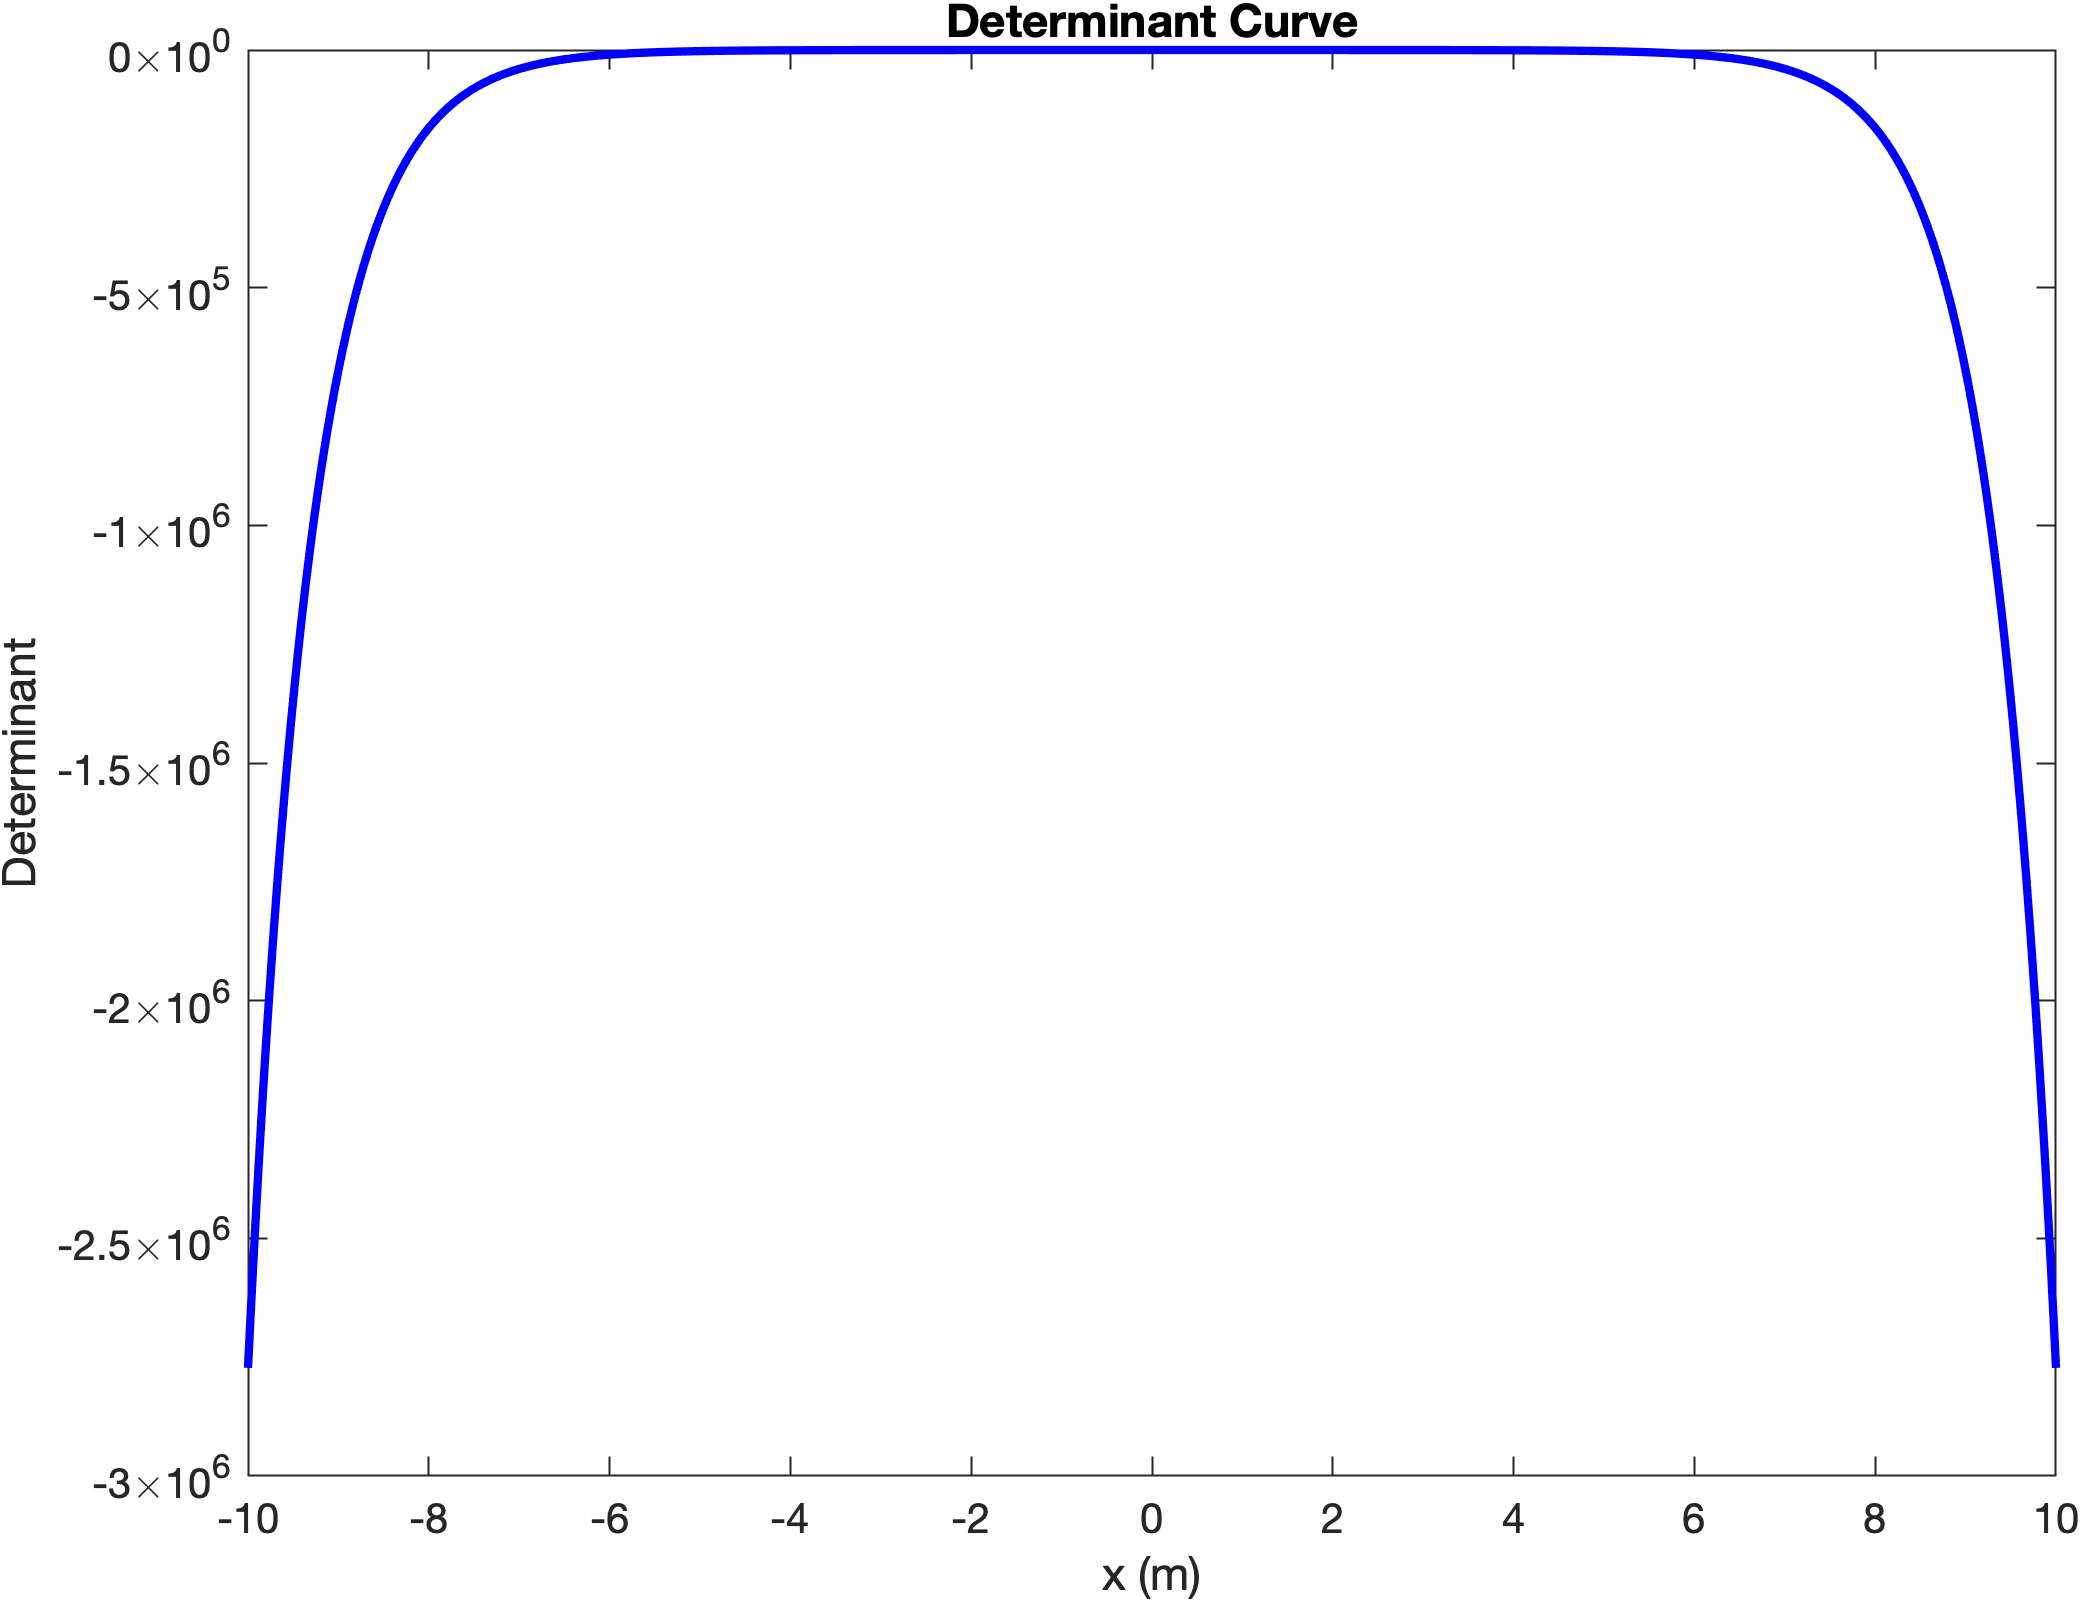
\includegraphics[height= 9.5cm, width= 12.5cm]{curve_Determinant.png}
\caption{Determinant Curve}
\label{DeterminantCurve}
\end{figure}
Now that we know $X$ is invertible, we know that
\begin{equation}\label{eq:ConstantsAllEqualToZero}
    C_1=C_2=C_3=C_4=0.
\end{equation}

This shows us that Equation~\eqref{eq:SimplifiedSeparableSolutionNegativeX} will reduce to
\begin{equation}\label{eq:X=0}
    X=0,
\end{equation}
which again is a trivial solution.

This means that the only possible sign for the constant to be is positive. Now if the constant is positive, the separable solution is
\begin{equation}\label{eq:SeparableSolutionPositive}
    \centering
    \frac{X''''(x)}{X(x)} = -\frac{1}{k^2}\frac{\ddot{T}(t)}{T(t)} = \lambda
\end{equation}
where

\centerline{$\lambda=\beta^4$.}

Looking at the equation for spatial dependence, we have
\begin{equation}\label{eq:SpatialDependence}
    \centering
    \frac{X''''(x)}{X(x)} = \beta^4.
\end{equation}
Multiplying both sides of Equation~\eqref{eq:SpatialDependence} by $X(x)$ and then subtracting the right side of Equation~\eqref{eq:SpatialDependence}, we obtain
\begin{equation}\label{eq:SimplifiedSpatialDependence}
    \centering
    X''''(x)-\beta^4X(x)=0.
\end{equation}
Looking at the equation for time dependence, we have
\begin{equation}\label{eq:TimeDependence}
    \centering
    -\frac{1}{k^2}\frac{\ddot{T}(t)}{T(t)} = \beta^4.
\end{equation}
Multiplying both sides of Equation~\eqref{eq:TimeDependence} by $-k^2T(t)$ and then adding the right side of Equation~\eqref{eq:TimeDependence}, we obtain
\begin{equation}\label{eq:SimplifiedTimeDependence}
    \centering
    \ddot{T}(t)+k^2\beta^4T(t) = 0.
\end{equation}
Equation~\eqref{eq:SimplifiedTimeDependence} is equivalent to the equation for the simple harmonic oscillator
\begin{equation}\label{eq:SimpleHarmonicoscillator}
    \centering
    \ddot{x}+w^2x = 0,
\end{equation}
where
\begin{equation}\label{eq:OmegaRelation}
    \centering
    w=k\beta^2.
\end{equation}
Equation~\eqref{eq:SimpleHarmonicoscillator} simplifies to  
\begin{equation}\label{eq:GeneralSolution}
    \centering
    T(t)=Ecos(k\beta^2t)+F\sin(k\beta^2t),
\end{equation}
where E and F are constants.

Taking the derivative of Equation~\eqref{eq:GeneralSolution}, we obtain
\begin{equation}\label{eq:GeneralSolutionInitialConditions}
    \centering
    \dot{T}(t)=-k\beta^2tEsin(k\beta^2t)+k\beta^2tFcos(k\beta^2t).
\end{equation}
Recall Equation~\eqref{eq:SimplifiedInitialCondition2} Replacing $t$ with $0$, we are left with
\begin{equation}\label{eq:GeneralSolutionAnswer}
    \centering
    k\beta^2F=0.
\end{equation}
We know that $\beta\neq0$ because the separation constant is positive. Furthermore, we know that $k\neq0$ because we are dividing by $k$ in Equation~\eqref{eq:TimeDependence}. It is impossible to divide by 0, thus we can conclude that \\

\centerline{$F=0$.}

Due to the fact that $F=0$, Equation~\eqref{eq:GeneralSolutionInitialConditions} simplifies to 
\begin{equation}\label{eq:SimplifiedGeneralSolutionInitialConditions}
    \centering
    \dot{T}(t)=-k\beta^2tEsin(k\beta^2t).
\end{equation}
Now, we must prove that the general solution for $X$ is
\begin{equation}\label{eq:FinalGeneralSolution}
    \centering
    X(x)=A^*cos(\beta x)+B^*sin(\beta x)+C^*cosh(\beta x)+D^*sinh(\beta x).
\end{equation}
To prove this, we need to plug Equation~\eqref{eq:FinalGeneralSolution} back into Equation~\eqref{eq:SimplifiedSpatialDependence}.

First, we need to determine the fourth derivative of Equation~\eqref{eq:FinalGeneralSolution} in order to substitute that back into Equation~\eqref{eq:SimplifiedSpatialDependence}.

The first derivative of Equation~\eqref{eq:FinalGeneralSolution} is
\begin{equation}\label{eq:FinalGeneralSolution'}
    \centering
    X'(x)=\beta(-A^*sin(\beta x)+B^*cos(\beta x)+C^*sinh(\beta x)+D^*cosh(\beta x)).
\end{equation}
The second derivative of Equation~\eqref{eq:FinalGeneralSolution} is
\begin{equation}\label{eq:FinalGeneralSolution''}
    \centering
    X''(x)=\beta^2(-A^*cos(\beta x)-B^*sin(\beta x)+C^*cosh(\beta x)+D^*sinh(\beta x)).
\end{equation}
The third derivative of Equation~\eqref{eq:FinalGeneralSolution} is
\begin{equation}\label{eq:FinalGeneralSolution'''}
    \centering
    X'''(x)=\beta^3(A^*sin(\beta x)-B^*cos(\beta x)+C^*sinh(\beta x)+D^*cosh(\beta x)).
\end{equation}
The fourth derivative of Equation~\eqref{eq:FinalGeneralSolution} is
\begin{equation}\label{eq:FinalGeneralSolution''''}
    \centering
    X''''(x)=\beta^4(A^*cos(\beta x)+B^*sin(\beta x)+C^*cosh(\beta x)+D^*sinh(\beta x)).
\end{equation}
Now that we have Equation~\eqref{eq:FinalGeneralSolution''''}, lets substitute it back into Equation~\eqref{eq:FinalGeneralSolution}
\begin{equation}\label{eq:SubstituteFinalGeneralSolution}
    \resizebox{.93\hsize}{!}
    {
        \centering
        \beta^4(A^*cos(\beta x)+B^*sin(\beta x)+C^*cosh(\beta x)+D^*sinh(\beta x)-(A^*cos(\beta x)+B^*sin(\beta x)+C^*cosh(\beta x)+D^*sinh(\beta x))=0.
    }
\end{equation}
After substituting, we know that Equation~\eqref{eq:SubstituteFinalGeneralSolution} proves that Equation~\eqref{eq:FinalGeneralSolution} is the general solution for $X$.

Now that we have the correct general solution, we will enforce our boundary conditions to determine the admissible values of the separation constant.

Recall Equation~\eqref{eq:SimplifiedBoundaryConditionX}. Replacing $x$ with $0$ into Equation~\eqref{eq:FinalGeneralSolution}, we obtain
\begin{equation}\label{eq:FinalGeneralSolutionBoundaryConditionX}
    \centering
    A^*+C^*=0.
\end{equation}
Recall Equation~\eqref{eq:SimplifiedBoundaryConditionX'}. Replacing $x$ with $0$ into Equation~\eqref{eq:FinalGeneralSolution'}, we obtain
\begin{equation}\label{eq:FinalGeneralSolutionBoundaryConditionX'}
    \centering
    B^*+D^*=0.
\end{equation}
Recall Equation~\eqref{eq:SimplifiedBoundaryConditionX''}. Replacing $x$ with $L^*$ into Equation~\eqref{eq:FinalGeneralSolution''}, we obtain
\begin{equation}\label{eq:FinalGeneralSolutionBoundaryConditionX''}
    \centering
    -A^*cos(\beta L^*)-B^*sin(\beta L^*)+C^*cosh(\beta L^*)+D^*sinh(\beta L^*)=0.
\end{equation}
Recall Equation~\eqref{eq:SimplifiedBoundaryConditionX'''}. Replacing $x$ with $L^*$ into Equation~\eqref{eq:FinalGeneralSolution'''}, we obtain
\begin{equation}\label{eq:FinalGeneralSolutionBoundaryConditionX'''}
    \centering
    A^*sin(\beta L^*)-B^*cos(\beta L^*)+C^*sinh(\beta L^*)+D^*cosh(\beta L^*)=0.
\end{equation}
**Note: We can divide $\beta$ to simplify Equations~\eqref{eq:FinalGeneralSolution'} through~\eqref{eq:FinalGeneralSolution'''}.

Solving for $C^*$ and $D^*$ in Equations~\eqref{eq:FinalGeneralSolutionBoundaryConditionX} and~\eqref{eq:FinalGeneralSolutionBoundaryConditionX'}, we obtain
\begin{equation}\label{eq:IsolateFinalGeneralSolutionBoundaryConditionX}
    \centering
    C^*=-A^*
\end{equation}
and
\begin{equation}\label{eq:IsolateFinalGeneralSolutionBoundaryConditionX'}
    \centering
    D^*=-B^*,
\end{equation}
respectively.

We can now eliminate $C^*$ and $D^*$ from Equations~\eqref{eq:FinalGeneralSolutionBoundaryConditionX''} and~\eqref{eq:FinalGeneralSolutionBoundaryConditionX'''}.

Substituting Equations~\eqref{eq:IsolateFinalGeneralSolutionBoundaryConditionX} and~\eqref{eq:IsolateFinalGeneralSolutionBoundaryConditionX'} into Equation~\eqref{eq:FinalGeneralSolution'''}, we obtain
\begin{equation}\label{eq:ReplacedFinalGeneralSolution'''}
    \centering
    -A^*cos(\beta L^*)-B^*sin(\beta L^*)-A^*cosh(\beta L^*)-B^*sinh(\beta L^*)=0.
\end{equation}
Simplifying Equation~\eqref{eq:ReplacedFinalGeneralSolution'''}, we obtain
\begin{equation}\label{eq:SimplifiedReplacedFinalGeneralSolution'''}
    \centering
    A^*(cos(\beta L^*)+cosh(\beta L^*))=-B^*(sin(\beta L^*)+sinh(\beta L^*))=0.
\end{equation}
Solving for $A^*$ in Equation~\eqref{eq:SimplifiedReplacedFinalGeneralSolution'''}, we obtain
\begin{equation}\label{eq:SolveASimplifiedReplacedFinalGeneralSolution'''}
    \centering
    A^*=-B^*\frac{(sin(\beta L^*)+sinh(\beta L^*))}{(cos(\beta L^*)+cosh(\beta L^*))}.
\end{equation}

Substituting Equations~\eqref{eq:IsolateFinalGeneralSolutionBoundaryConditionX} and~\eqref{eq:IsolateFinalGeneralSolutionBoundaryConditionX'} into Equation~\eqref{eq:FinalGeneralSolution''''}, we obtain
\begin{equation}\label{eq:ReplacedFinalGeneralSolution''''}
    \centering
    A^*sin(\beta L^*)-B^*cos(\beta L^*)-A^*sinh(\beta L^*)-B^*cosh(\beta L^*)=0.
\end{equation}

Using Equation~\eqref{eq:SolveASimplifiedReplacedFinalGeneralSolution'''} we can get Equation~\eqref{eq:ReplacedFinalGeneralSolution''''} in terms of $B$.
\begin{equation}\label{eq:AReplacedFinalGeneralSolution''''}
    \resizebox{.91\hsize}{!}
    {
        \centering
        -B^*sin(\beta L^*)\frac{(sin(\beta L^*)+sinh(\beta L^*))}{(cos(\beta L^*)+cosh(\beta L^*))}-B^*cos(\beta L^*)+B^*sinh(\beta L^*)\frac{(sin(\beta L^*)+sinh(\beta L^*))}{(cos(\beta L^*)+cosh(\beta L^*))}-B^*cosh(\beta L^*)=0.
    }
\end{equation}
Combining like terms from Equation~\eqref{eq:AReplacedFinalGeneralSolution''''}, we obtain
\begin{equation}\label{eq:CombineLikeTermsReplacedFinalGeneralSolution''''}
    \centering
    B^*(sinh(\beta L^*)-sin(\beta L^*))\frac{(sin(\beta L^*)+sinh(\beta L^*))}{(cos(\beta L^*)+cosh(\beta L^*))}=B^*(cos(\beta L^*)+cosh(\beta L^*)).
\end{equation}
Multiplying $(cos(\beta L^*)+cosh(\beta L^*))$ and cancelling $B^*$ from both sides of Equation~\eqref{eq:CombineLikeTermsReplacedFinalGeneralSolution''''}, we obtain
\begin{equation}\label{eq:IsolatesincosReplacedFinalGeneralSolution''''}
    \resizebox{.91\hsize}{!}
    {
        \centering
        (sin(\beta L^*)+sinh(\beta L^*))(sinh(\beta L^*)-sin(\beta L^*))=(cos(\beta L^*)+cosh(\beta L^*))(cos(\beta L^*)+cosh(\beta L^*)).
    }
\end{equation}
Factoring the polynomials on both sides of Equation~\eqref{eq:IsolatesincosReplacedFinalGeneralSolution''''}, we obtain 
\begin{equation}\label{eq:FactorReplacedFinalGeneralSolution''''}
    \centering
    (-sin^2(\beta L^*)+sinh^2(\beta L^*))=(cos^2(\beta L^*)+2cos(\beta L^*)cosh(\beta L^*)+cosh^2(\beta L^*)).
\end{equation}
Simplifying Equation~\eqref{eq:FactorReplacedFinalGeneralSolution''''}, we obtain
\begin{equation}\label{eq:SimplifyFactorReplacedFinalGeneralSolution''''}
    \centering
    -(cosh^2(\beta L^*)-sinh^2(\beta L^*))=(sin^2(\beta L^*)+cos^2(\beta L^*)+2cos(\beta L^*)cosh(\beta L^*)).
\end{equation}
Replacing $(cosh^2(\beta L^*)-sinh^2(\beta L^*))$ in Equation~\eqref{eq:SimplifyFactorReplacedFinalGeneralSolution''''} with 1 we obtain,
\begin{equation}\label{eq:HyperbolicReplacedFinalGeneralSolution''''}
    \centering
    -1=(sin^2(\beta L^*)+cos^2(\beta L^*)+2cos(\beta L^*)cosh(\beta L^*)).
\end{equation}
Replacing $((sin^2(\beta L^*)+cos^2(\beta L^*))$ in Equation~\eqref{eq:HyperbolicReplacedFinalGeneralSolution''''} with 1 we obtain, 
\begin{equation}\label{eq:TrigonometricReplacedFinalGeneralSolution''''}
    \centering
    -1=-1+2cos(\beta L^*)cosh(\beta L^*)).
\end{equation}
Making one last simplification, we satisfy the transcendental equation,
\begin{equation}\label{eq:FinalTranscendentalEquation}
    \centering
    cos(\beta L^*)cosh(\beta L^*)=-1.
\end{equation}
The plot for Equation~\eqref{eq:FinalTranscendentalEquation} is shown in Figure~\ref{FundamentalFrequency}. The roots for Equation~\eqref{eq:FinalTranscendentalEquation} are marked as red x's. 
\begin{figure}[H]
\centering
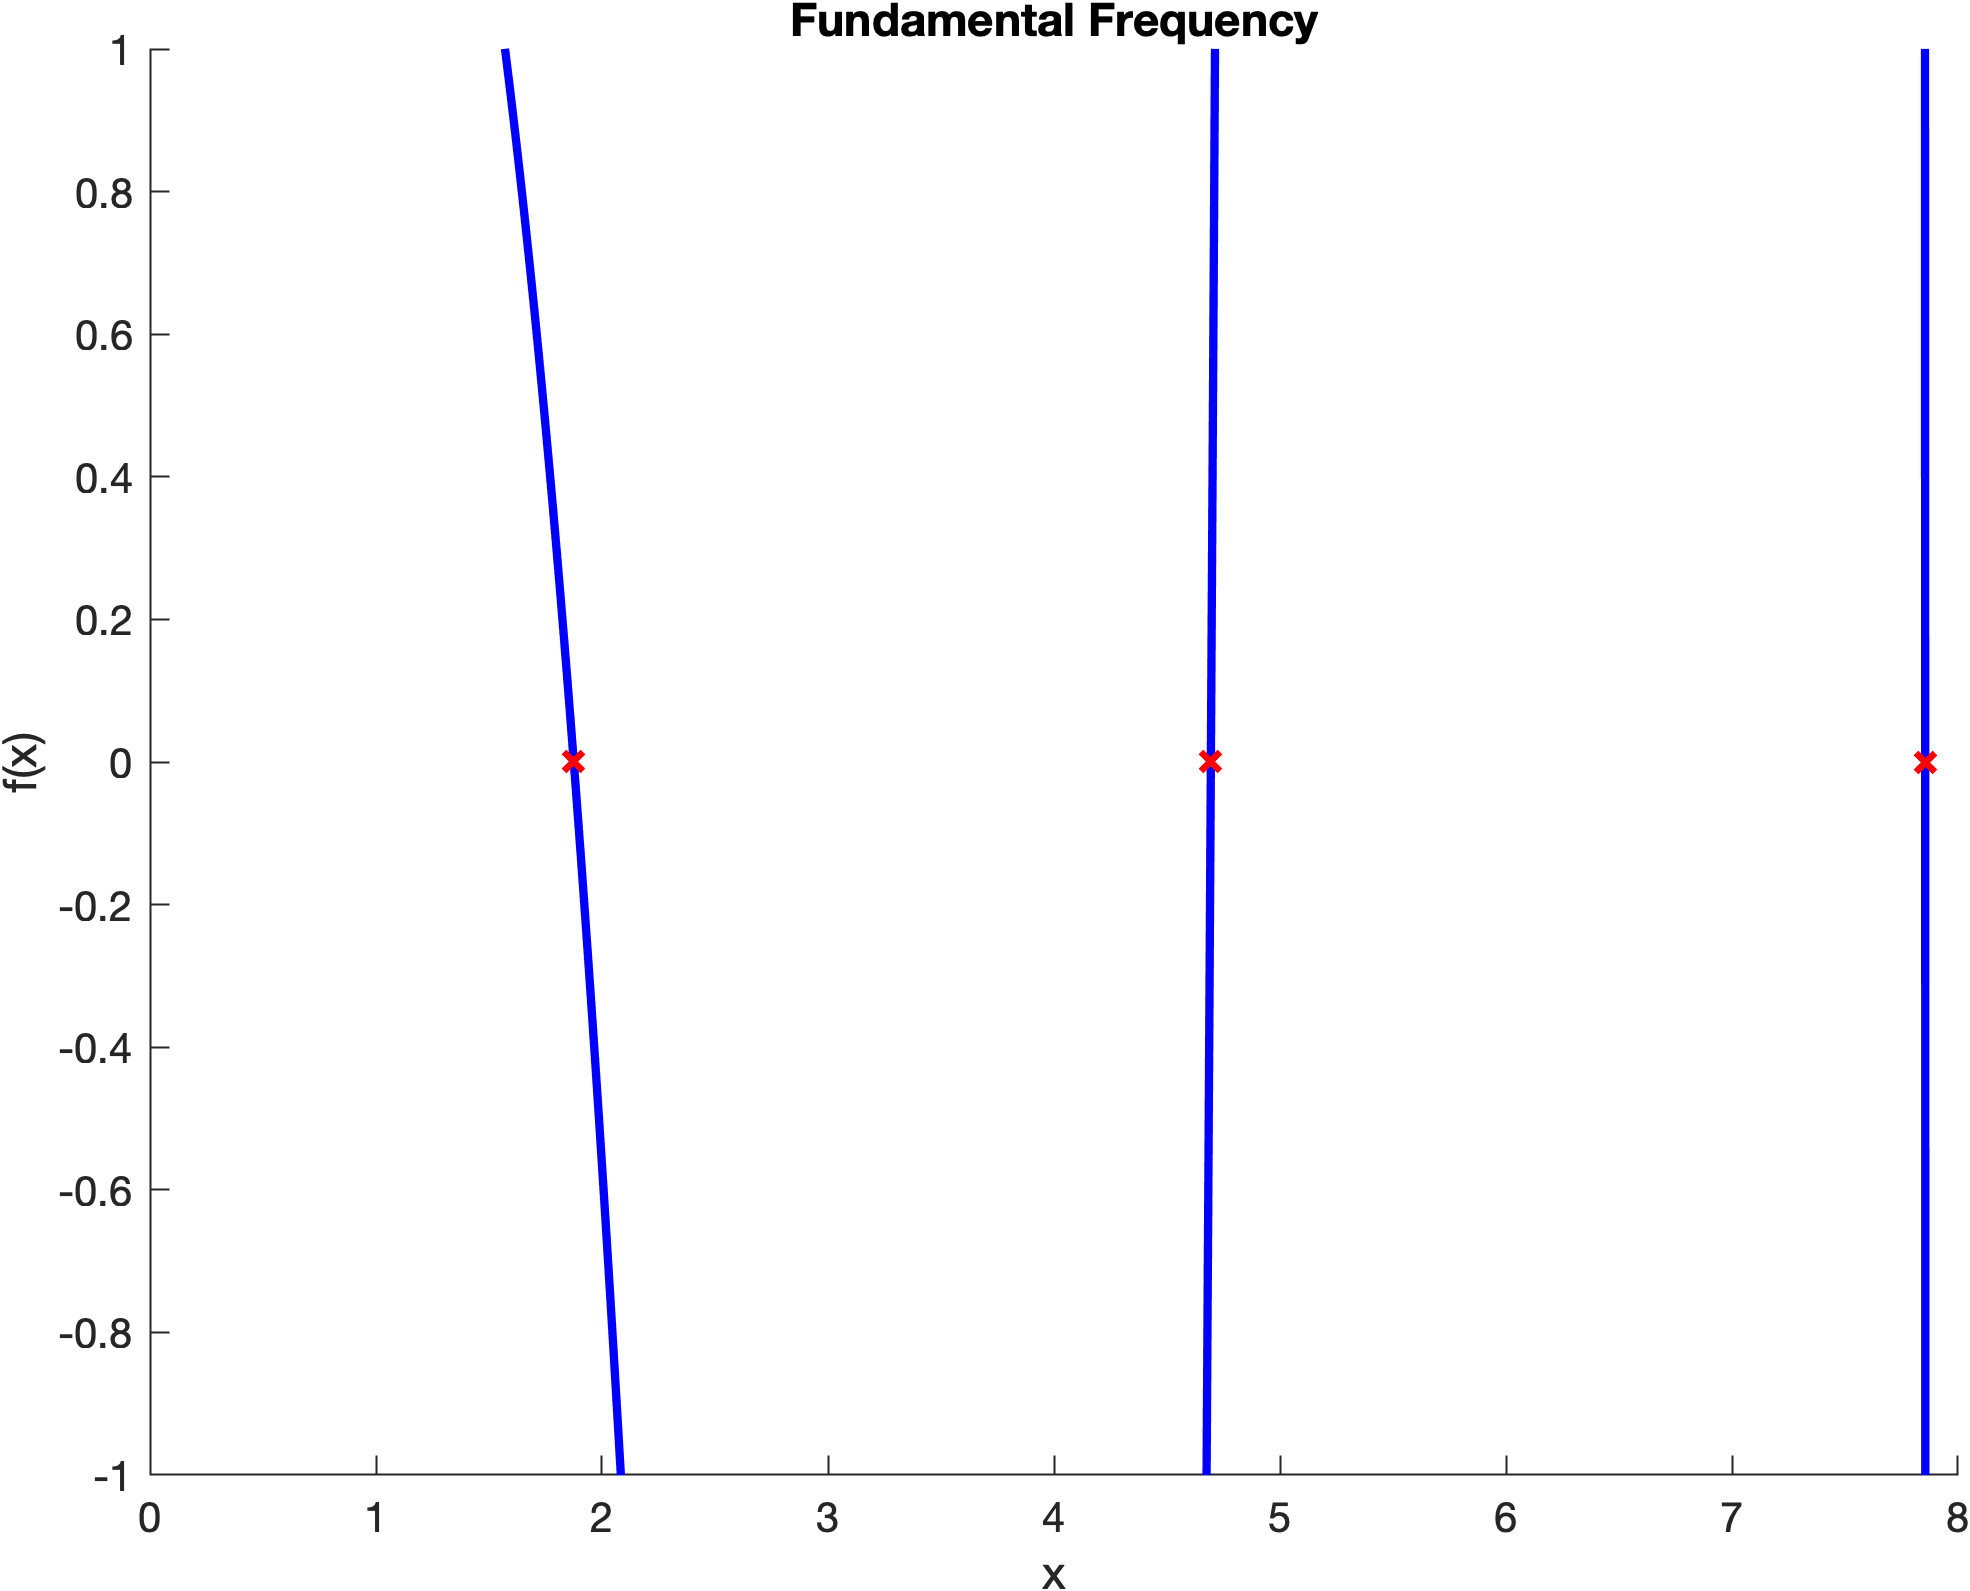
\includegraphics[height= 9.5cm, width= 12.5cm]{curve_Fundamenal_Frequency.png}
\caption{Fundamental Frequency}
\label{FundamentalFrequency}
\end{figure}
Now that we have satisfied Equation~\eqref{eq:FinalTranscendentalEquation}, we will use Newton's Method to solve for first three non-zero roots
\begin{equation}\label{eq:RootsEquationX1}
    \centering
    x_1=\beta_1\cdot L^*,
\end{equation}
\begin{equation}\label{eq:RootsEquationX2}
    x_2=\beta_2\cdot L^*,
\end{equation}
\begin{equation}\label{eq:RootsEquationX3}
    x_3=\beta_3\cdot L^*.
\end{equation}
We can use Equations~\eqref{eq:RootsEquationX1} through~\eqref{eq:RootsEquationX3} to solve for the associated $\beta$ value for the fundamental frequency, then plug the $\beta$ values into Equation~\eqref{eq:OmegaRelation}.

To solve for the fundamental frequency, we used 
\begin{equation}\label{eq:FundamentalFrequency}
    \omega_1=(\frac{x_1}{L^*})^2\sqrt{\frac{EI_0}{\rho A_0}}\cdot\frac{1}{2\pi},
\end{equation}
where $\omega_1$ is the fundamental frequency, $x_1$ is the non-zero root, and $\rho$ is the density. We calculated $\omega_1$ to be 235.6927 Hz.

Estimating $\omega_2$ in terms of $E$, $I_0$, $\rho$, $A_0$, and $L^*$, we use
\begin{equation}\label{eq:NaturalFrequency2}
    \omega_2=(\frac{4.6941}{L^*})^2\sqrt{\frac{EI_0}{\rho A_0}}\cdot\frac{1}{2\pi}.
\end{equation}
Estimating $\omega_3$ in terms of $E$, $I_0$, $\rho$, $A_0$, and $L^*$, we use
\begin{equation}\label{eq:NaturalFrequency2}
    \omega_3=(\frac{7.8548}{L^*})^2\sqrt{\frac{EI_0}{\rho A_0}}\cdot\frac{1}{2\pi}.
\end{equation}
\newpage
\section{Cost}
The total mass of the antenna is 0.0182 kilograms. This was calculated by multiplying the density times the volume. The cost of stainless steel is approximately \$0.23 per kilogram [4]. The cost of the stainless steel for the antenna design is \$0.0042.
\newpage

\section{Conclusion}
For the antenna design the material that was used is stainless steel 304. Stainless steel 304 has a density of 8000 kg/m$^3$ [2], an elastic modulus of 200 GPa [2] and a yield strength of 207 MPa [3]. Geometrically, this design has 6 segments. When fully extended the length of the antenna is 69.5 centimeters and when fully retracted the length is 11.583 centimeters. The tube wall thickness is 0.0417  centimeters, and the maximum diameter is 0.5 centimeters. The cost of the raw material is \$0.0042 with the mass of our antenna being 0.0182 kilograms. The maximum normal stress under given loading is 167.815 MPa. The maximum deflection under given loading is 0.067103 meters. With a concentrated force of 1.7849 Newtons acting at 46.333 centimeters from the fixed end of the antenna, the factor of safety is 1.2335 (dimension-less). While choosing the design, we wanted to minimize cost while maintaining a design that had a factor of safety of at least 1.2. The fundamental frequency of vibration of our antenna is 235.69 Hz. When finding the geometry, the length was decreased to the lowest length that can still permit an FM radio signal and determined $h$ by dividing the radius by the number of segments. By inputting different numbers of segments, we were able to monitor the change in the factor of safety and come to a lower value that still meets design parameters.
\newpage

\section{References}
[1] Y. Zhang, Z. Yang, L. Deng and S. Li, “Research on Wireless Positioning Technology Based on Digital FM Broadcasting”, International Journal of Digital
Multimedia Broadcasting, vol. 2019, Article ID 1051386, 10 pages, 2019.v

[2] H. M. Cobb, “History of Stainless Steel: Two New Classes
of Stainless Steel.” 1st ed. Ohio: A S M International, 2010.

[3] Thyssenkrupp Materials LTD, C. Lane, C. Heath, West    Midlands, “Stainless Steel 304 1.4301,” Jan. 2018. Accesses on: Oct. 11, 2021. [Online]. Available:          https://www.thyssenkrupp-materials.co.uk/stainless-steel-304-14301.html

[4] “Stainless Steel: 304 SS,” [Online]. Available: https://www.scrapmonster.com/scrap/304-ss/48
\newpage

\section{Appendix A: Design Specification Form}
\begin{figure}[H] 
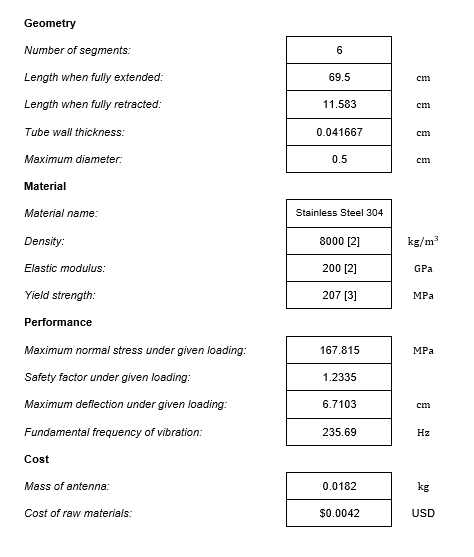
\includegraphics[height= 21.5cm, width= 17.5cm]{Appendix_A.png}
\end{figure}
\newpage

\section{Appendix B: Authorship Declaration Form} 
\begin{figure}[H]
\centering
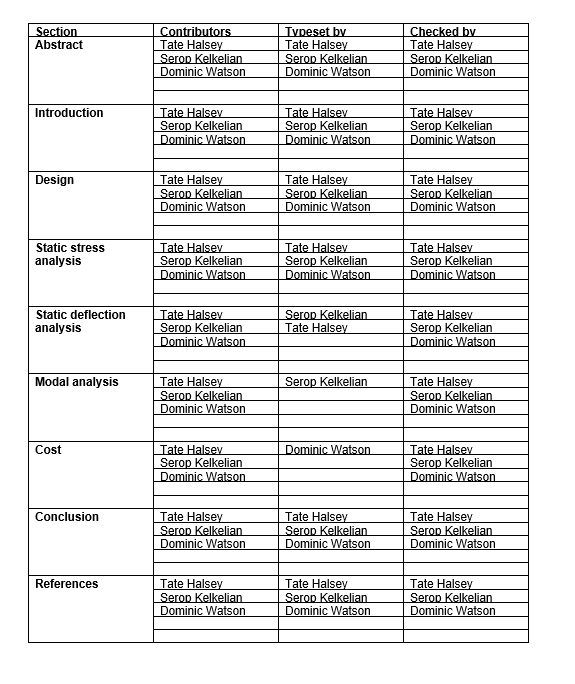
\includegraphics[height= 20.5cm, width= 18.5cm]{Appendix_B.png}
\end{figure}
\newpage

\section{Appendix C: MATLAB Script}
\lstinputlisting[style = Matlab-editor]{projectScripts.m}
\newpage

\end{document}